\section{Problem 1, Parsing}
\subsection{a) What is the difference between a top-down parser and a bottom-up parser?}
% bottom-up parsing: pg 233
% top-down parsing: pg 61
A top-down parser begins with the grammar's starting symbol and tries to figure out what `moves' were taken to get from it to the input string.

Bottom-up parsers begin with the first terminal of the input and works backwards from it towards the grammar's starting symobl.


\subsection{b) What is the difference between a LL parser and a LR parser?}
% LL parser is a predictive parser, pg 64-8, 222-231
% LR parser, pg 53-252, 275-7
% A derivation of a string for a grammar is a sequence of grammar rule applications that transforms the start symbol into the string. A derivation proves that the string belongs to the grammar's language.

An LL parser parses the input from left to right and constructs a leftmost derivation of the sentence.
A leftmost derivation looks at the leftmost non-terminal first when deriving a string.

While LR parsers also parse the input from left to right, they construct a rightmost derivation of the sentence.
LR parsers are shift-reduce parsers.

Ohh, also while LR parsers \textit{can} be written by hand, they're typically not because it is a lot of work.


\section{Problem 2, Top-down parsing}
Consider the context free grammar:
\begin{table}[H]
\begin{tabular}{ccl}
	% ~ enters a nonbreaking space, which in this case just forces a space because LaTeX ignores the whitespace
	% between \textbar and whatever comes next
	A	& ::=	& aB \textbar ~D \textbar  ~F \\
	B 	& ::=	& bC \\
	C 	& ::=	& bC \textbar ~$\epsilon$ \\
	D  	& ::=	& EB \textbar ~dBEF \\
	E 	& ::=	& e \textbar ~$\epsilon$ \\
	F 	& ::=	& c \textbar ~f 
\end{tabular}
\end{table}

The grammar's terminals are \{a, b, c, d, e, f\}. \\
Its non-terminals are \{A, B, C, D, E, F\}.

\subsection{a) Tabulate the first and follow sets for the grammar.}
% the FIRST and FOLLOW sets are associated with some grammar.
% They allow us to choose which production to apply based on the next input symbol.
% FIRST(S) is the set of terminals that strings derived from S may with.
% FOLLOW(S), for a nonterminal S, is the set of terminals that can appear immediately to the right of S in some sentence
%
% Algorithm for FIRST(S):
	% if S is a terminal then FIRST(S) = {S}
	% if S ... the rest of it appears on pg 221 of the book
Using the method described on page 221-2 of \textsc{the Dragon Book} to find the \textsc{first} and \textsc{follow} sets.
I think it's easier if we start with the non-terminals that only have terminals in their productions.
% oh, okay so the greek letters in the book can be empty, according to 4.2.2 "notational conventions" on pg 199
% they also mean any string of grammar symbols, so they can represent non-terminals. That makes stuff easier.
% wait ok so since the greek letters can be empty, that means that A -> B matches A-> aBb (lowercase is greek here) and A-> aB
% also in A -> dBEF == A -> aF (a = dBE), or A -> dBb (b = EF).
% fucking sheesh

All right well I did that on paper here is the tabulated result:

\begin{table}[H]
\begin{center}
\begin{tabular}{l|l|l}
\hline
	Symbol	& \textsc{first}		& \textsc{follow} \\ \hline \hline
	A		& \{a, d, e, b, c, f\}	& \{\$\} \\
	B 		& \{b\}					& \{\$, e, c, f\}\\
	C		& \{b, $\epsilon$\}		& \{\$, e, c, f\}\\
	D		& \{d, e, b\}			& \{\$\}\\
	E		& \{e, $\epsilon$\}		& \{b, c, f\}\\
	F		& \{c, f \}				& \{\$\}\\
	a		& \{a\}					& $\emptyset$ \\
	b		& \{b\}					& $\emptyset$\\
	c		& \{c\}					& $\emptyset$\\
	d		& \{d\}					& $\emptyset$\\
	e		& \{e\}					& $\emptyset$\\
	f		& \{f\}					& $\emptyset$\\ \hline
\end{tabular}
\label{tab:2a}
\caption{\textsc{first} and \textsc{follow} sets for the Problem 2 grammar.}
\end{center}
\end{table}

\subsection{b) Construct the predictive parsing table for the grammar.}
There's an algorithm for that (Algorithm 4.31 in \textsc{ye olde booke of dragons}.)
%algo 4.31 is basically "for each production <nonterminal> -> <string of symbols>, do:
%stuff!



\begin{table}[H]
\begin{center}
\begin{tabular}{c|c|c|c|c|c|c|c}
	\hline \hline 
	\multirow{2}{*}{\textsc{Non-Terminal}} & \multicolumn{7}{ c }{\textsc{Input Symbol}} \\ \cline{2-8} % cline 2-8 is like \hline 'cept only for column 2-8
	 	& a 			   & b 				 & c 			   & d 	 			 & e 			   & f 				 & \$ \\ \hline
	A 	& A$\rightarrow$aB & A$\rightarrow$D & A$\rightarrow$F & A$\rightarrow$D & A$\rightarrow$D & A$\rightarrow$F & 	  \\ \hline
	B	& 				   & B$\rightarrow$bC&				   &				 &				   &				 &	  \\ \hline
	C	&				   & C$\rightarrow$bC& C$\rightarrow \epsilon$ & 		 &C$\rightarrow \epsilon$ &C$\rightarrow \epsilon$&C$\rightarrow\epsilon$\\\hline
	D 	&				   & D$\rightarrow$EB & & D$\rightarrow$dBEF & D$\rightarrow$EB & &D$\rightarrow$EB \\ \hline
	E 	& 				   & E$\rightarrow\epsilon$ & E$\rightarrow\epsilon$ & & E$\rightarrow$e &E$\rightarrow\epsilon$ & \\ \hline
	F 	& 				   &			     & F$\rightarrow$c			  & & & F$\rightarrow$f & \\ \hline
% see http://en.wikibooks.org/wiki/LaTeX/Tables#Columns_spanning_multiple_rows for how to make it span multiple rows or whatever, bro.	
\end{tabular}
\caption{Predictive parsing table for the Problem 2 grammar.}
\label{tab:2b}
\end{center}
\end{table}


\subsection{c) Show the moves a predictive, nonrecursive parser would make on the input: dbbbf. 
Make sure to show the matched part of the input, the parser's stack, the remaining input and the action taken at each step.}
Again there is an algorithm for this in \textsc{book: Dragon, Purple}.
It is ``Algorithm 4.34'' and you can find it on page 226.

The notation I've used in table~\ref{tab:2c} is slightly different than the one seen in Figure 4.21 on page 228 in the book:
in table~\ref{tab:2c}, the action listed in row $n$ has been performed in row $n+1$.


\begin{table}[H]
\begin{center}
\begin{tabular}{lrrl}
	\hline \hline
	\textsc{Matched} & \textsc{Stack} 	& \textsc{Input}	& \textsc{Action}	\\ \hline
					 & A\$				& dbbbf\$			& Output A$\rightarrow$D		\\
					 & D\$				& dbbbf\$			& Output D$\rightarrow$dBEF	\\
					 & dBEF\$			& dbbbf\$			& Match d		  	\\ 
	d				 & BEF\$			& bbbf\$			& Output B$\rightarrow$bC		\\
	d				 & bCEF\$			& bbbf\$			& Match b			\\
	db				 & CEF\$			& bbf\$				& Output C$\rightarrow$bC		\\
	db				 & bCEF\$			& bbf\$				& Match b			\\
	dbb				 & CEF\$			& bf\$				& Output C$\rightarrow$bC		\\
	dbb				 & bCEF\$			& bf\$				& Match b			\\
	dbbb			 & CEF\$			& f\$				& Output C$\rightarrow\epsilon$		\\
	dbbb			 & EF\$				& f\$				& Output E$\rightarrow\epsilon$		\\
	dbbb			 & F\$				& f\$				& Output F$\rightarrow$f		\\
	dbbb			 & f\$				& f\$				& Match f			\\
	dbbbf			 & \$				& \$				& 					\\ \hline					
\end{tabular}
\caption{Moves made by a predictive parser for the Problem 2 grammar on the input string ``dbbbf''.}
\label{tab:2c}
\end{center}
\end{table}

\section{Problem 3, Bottom-up parsing}
Consider the context free grammar:

\begin{table}[H]
\begin{tabular}{ccl}
	% ~ enters a nonbreaking space, which in this case just forces a space because LaTeX ignores the whitespace
	% between \textbar and whatever comes next
	A	& ::=	& aB \textbar ~D \textbar ~F \\
	B 	& ::=	& Bb \textbar ~b \\
	D  	& ::=	& EB \textbar ~dBEF \\
	E 	& ::=	& e \\
	F 	& ::=	& c \textbar ~f \\
\end{tabular}
\caption{The Problem 3 grammar.}
\label{tab:3}
\end{table}


The grammar's terminals are \{A, B, D, E, F\} and its non-terminals are \{a, b, c, d, e, f\}.


\subsection{a) Construct the LR(0) automaton for this grammar.}
% Step 1. The items!
% (4.6.2, pg 242)
% no, no, Figure 4.33, man. Page 246.

% Step 1:
% 	Augment the grammar by adding A' -> A to it
% Step 2:
%	I_0 = Closure({[A' -> .A]})
%	Add I_0 to C
% Step 3:
%	For each I_i in C
%		for each grammar symbol X in I_i
%			if GOTO(I_i, X) is not empty and not in C)
%				add GOTO(I_i, X) to C 

% Each set in C is labeled I_i, where i = 0..n

% Essentially, it would seem that what we are looking for when we do
% Goto(I, X) are items in I that contain ".X"

Image depicted in Figure~\ref{fig:1-3-a} was made using \texttt{http://lucidchart.com}.

\begin{figure}[H]
\begin{center}
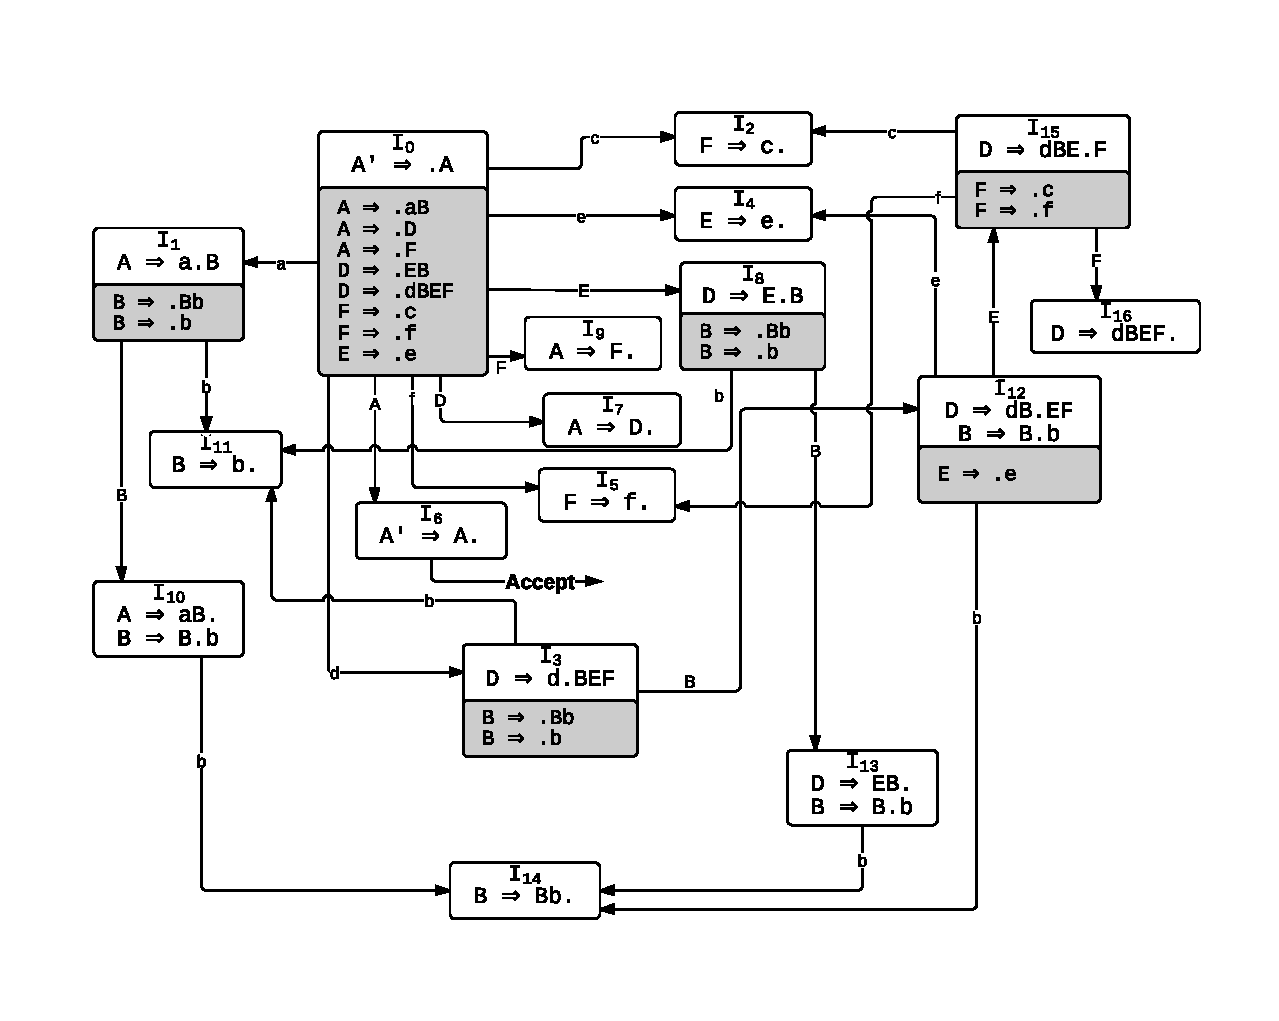
\includegraphics[width=\textwidth]{gfx/1-3-a.pdf}
\caption{The LR(0) Automaton for the Problem 3 grammar.}
\label{fig:1-3-a}
\end{center}
\end{figure}


